\documentclass[pt11,a4paper]{book}
\usepackage[utf8]{inputenc}
\usepackage{graphicx} 
\usepackage{amssymb,amsmath}
\usepackage[citecolor=black]{hyperref}
\usepackage{CJKutf8}


\begin{document}

\tableofcontents

\chapter{A Poem}
\section{The Cat}
\subsection{Sat On}
\subsubsection{The Mat}
\paragraph{Author}Chris

The \emph{slanty cat}

The \emph{\textbf{xxx}}

\textbf{Oh \underline{my} god}

The \textbf{fat cat}

The \underline{important cat}

The {\huge huge cat}

The {\large large cat}

The {\small small cat}

\begin{itemize} 
  \item VOCs
  \item CO$_2$
  \item NO$_2$
\end{itemize} 



\begin{enumerate} 
  \item A Cat 
  \item A Hat 
\end{enumerate} 



\begin{equation}
x + y = 7 \alpha,
\end{equation}



$\frac{ \Gamma }{ \sqrt{\gamma} }$

\paragraph{}

$\int_{0}^{\pi} \textrm{d}x \sin x$

\paragraph{}

$\int_{0}^{\cos x} \textrm{d} \log x$

\paragraph{}

$\lim_{x \to \infty} \log x$

\paragraph{}

$\sum\limits_{n=0}^{N}  n^{2}$

\paragraph{}

\$
\paragraph{}
\'{a}
\paragraph{}
$\vec{a}$
\paragraph{}
$\widehat{efg}$

\paragraph{}

\begin{figure}[t]
\centering
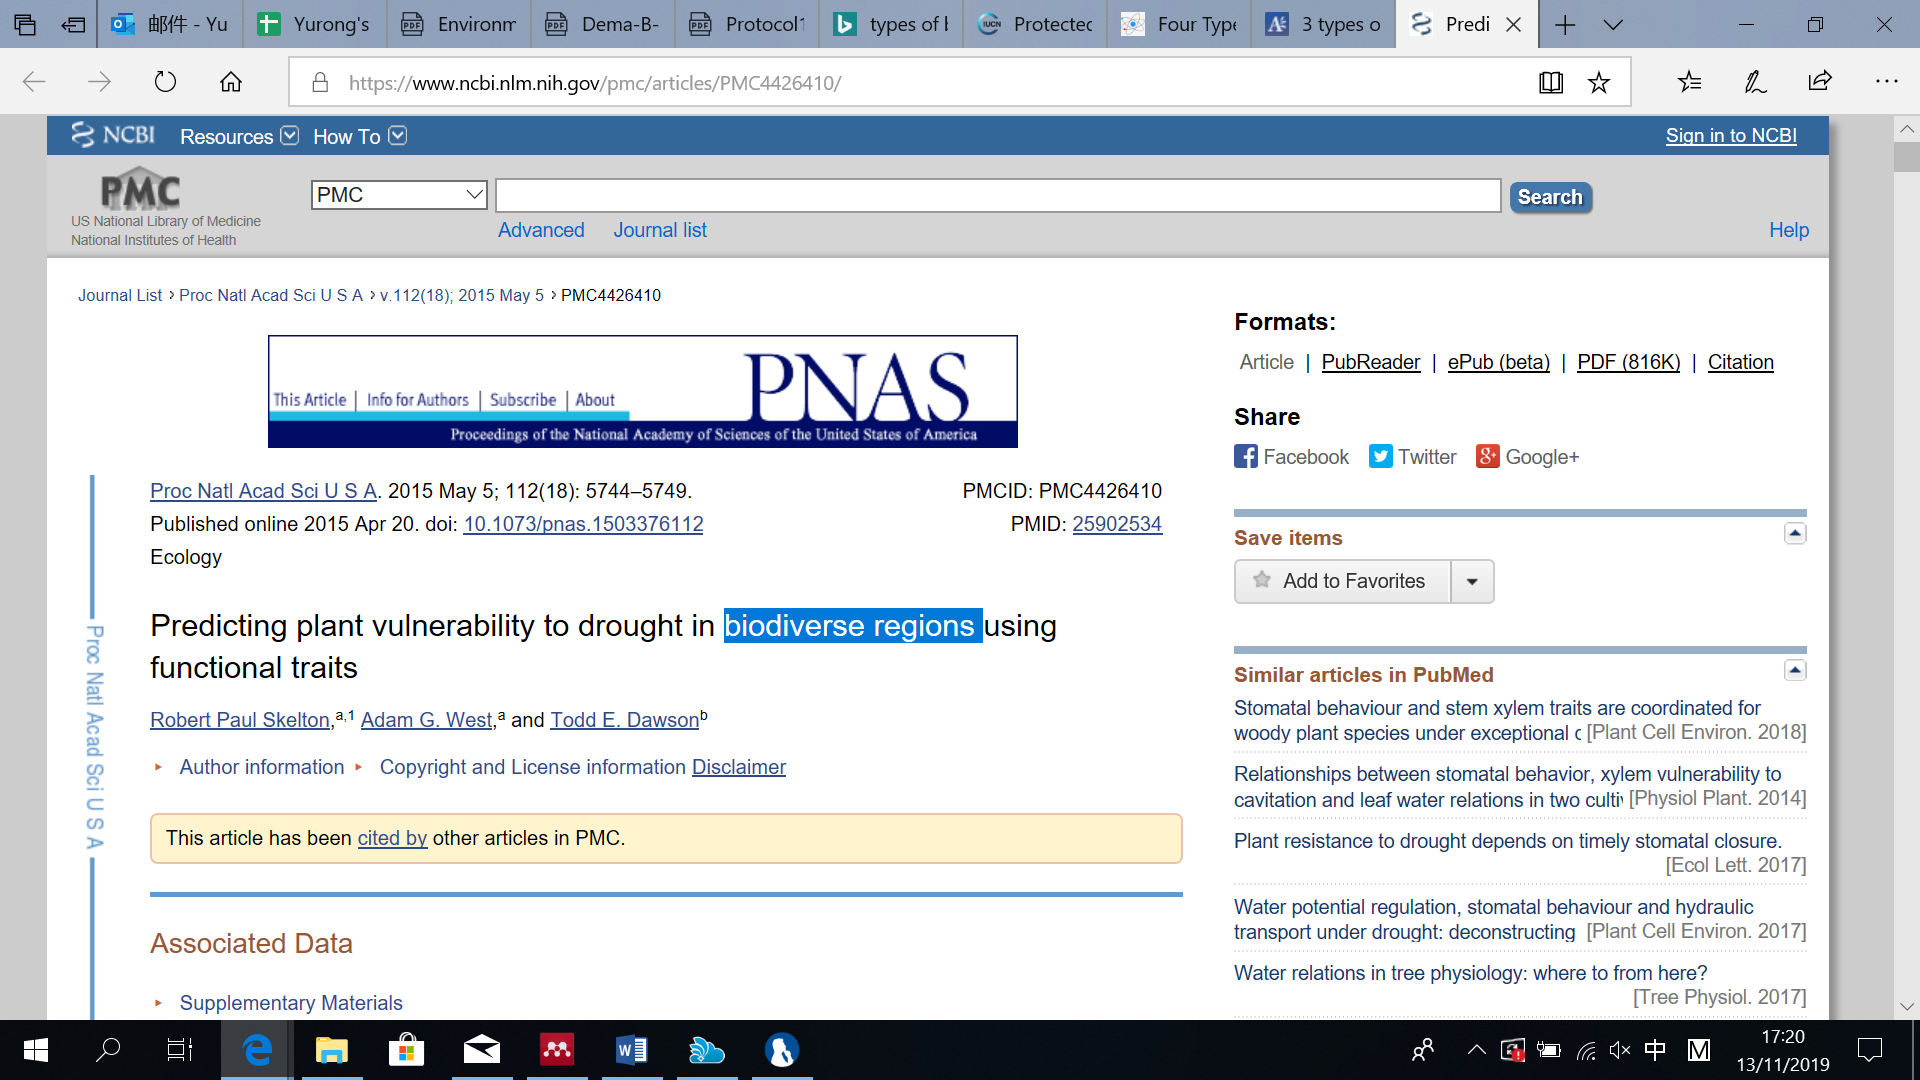
\includegraphics[scale=0.1]{Capture001.png}
\paragraph{}
\Caption{Capture}
\label{fig:galaxy}
\end{figure}

\paragraph{}

\begin{table}[h]
  \centering  
  \begin{tabular}{ l | c c c }    
      	&  X  &  Y  & Z\\   
    \hline    
    A	&  ax  & ay  & az\\ 
    B	&  bx  & by  & bz
  \end{tabular}  
\end{table}

\paragraph{}

\section{Referencing...}

\begin{equation}
x+y=7\alpha
\label{keyword1}
\end{equation}

...see \eqref{keyword1}... see Section \ref{sections}

\section{...Sections}\label{sections}


ridiculous claim \cite{fakenews}.
\begin{thebibliography}(1)
\bibitem[1]{fakenews}
"hklzh;kdhfe", 2013, xxx news

\end{thebibliography}

\paragraph{}

\begin{titlepage}

\begin{flushright}
right
\end{flushright}

\vspace{5cm}
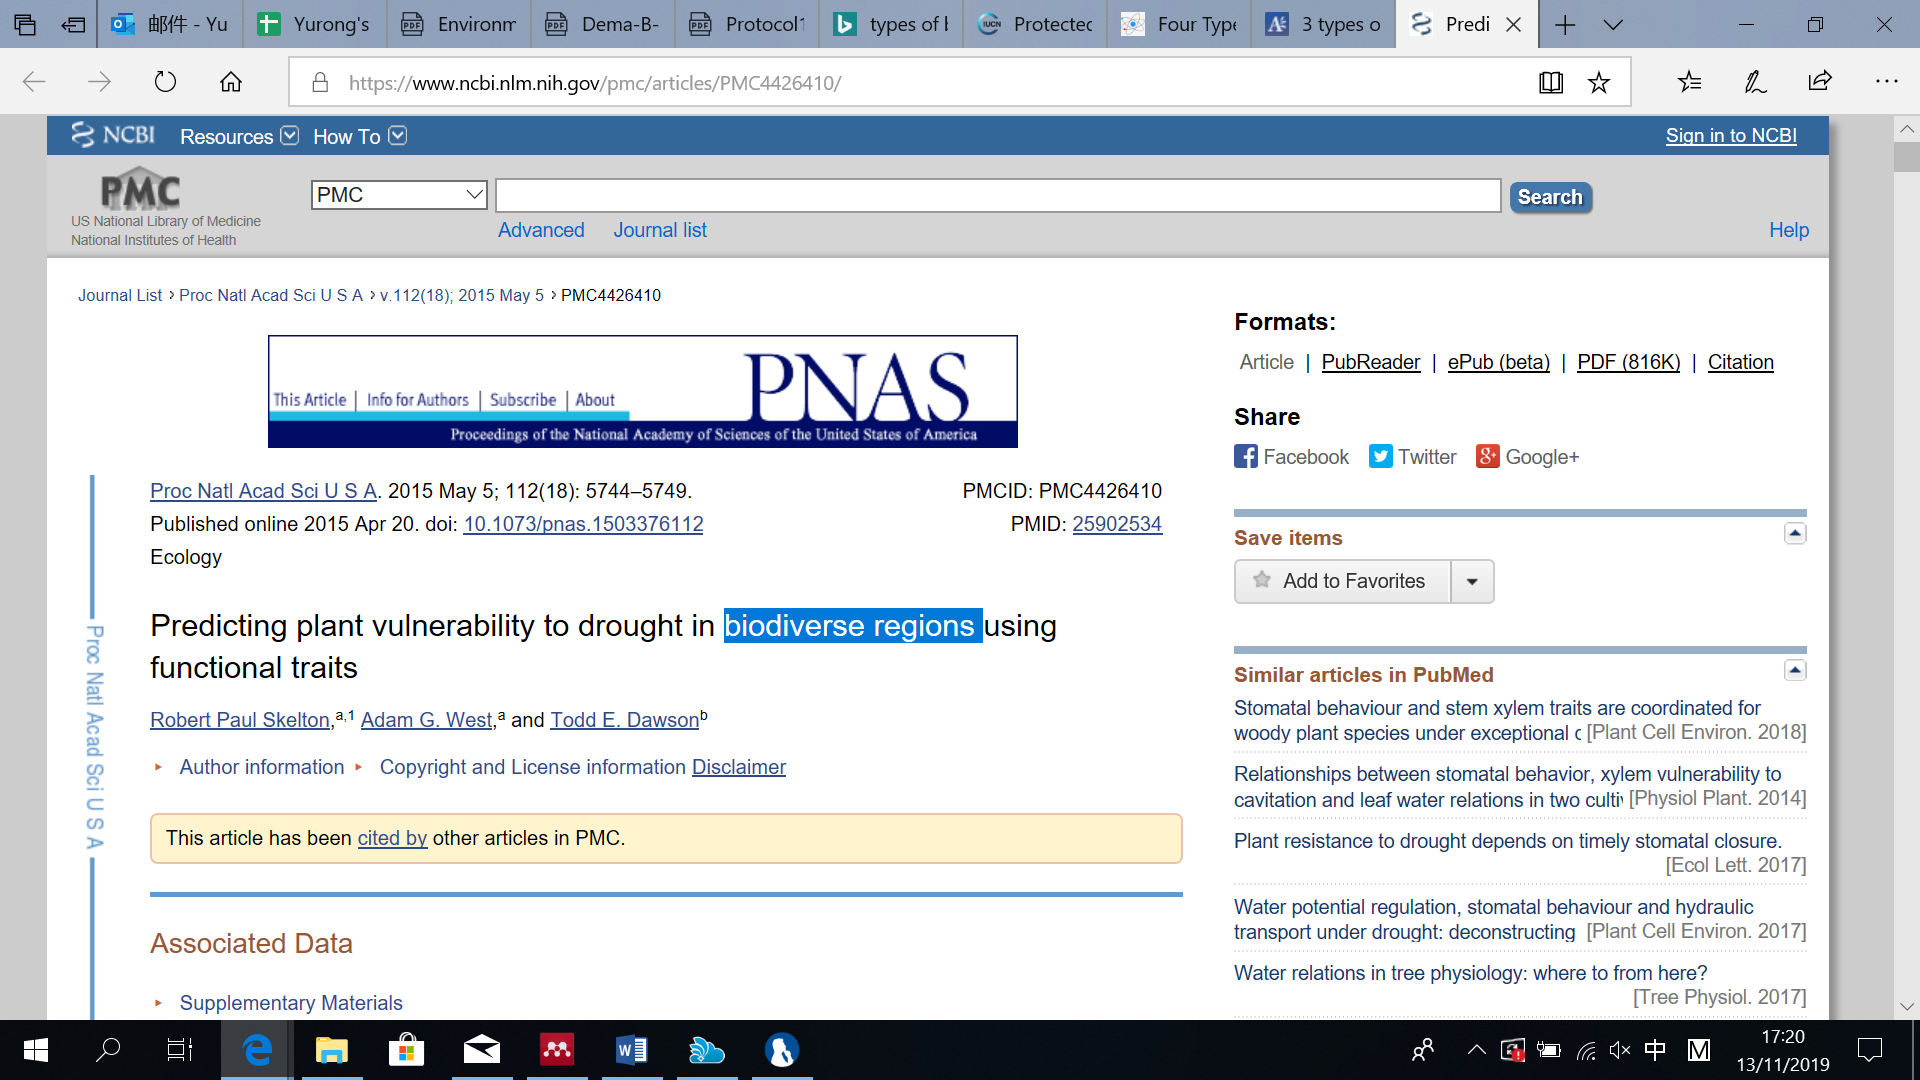
\includegraphics[width=5cm]{Capture001.png}

\begin{center}
center
\end{center}

\begin{flushleft}
left
\end{flushleft}

\end{titlepage}

\today

\paragraph{}

\end{document}
